Como se mencionó anteriormente, esta fase difiere entre el \hyperlink{abbr}{ML}
tradicional y el \hyperlink{abbr}{DL}. Mientras que en el primero nos enfocamos
a datos tabulares que tienen a ser abundantes, en el segundo nos comprometemos a
trabajar con pocos datos; por lo que la fase de preprocesamiento se enfocará más
a aumentar la base de datos, balancear las clases que la componen y lidiar con
detalles técnicos en la manipulación de vectores, matrices y tensores.

Debido a que en esta tesis trabajaremos con datos en imágenes y aplicamos
\hyperlink{abbr}{ConvNet}s que son capaces de aprender las características
importantes por si solas, podremos saltarnos las fases de ingeniería y selección
de características.

\subsection{Limpieza de datos}

Los archivos que contienen los datos y los procesos que generan los datos
también pueden incidir en ruido. Limpiar los datos se refiere a rellenar valores
faltantes utilizando técnicas de imputación de datos, estandarización y
normalización y también la remoción de valores inusuales.

En nuestro caso, debido a que la \hyperlink{abbr}{BD} esta pre-validada. No es
necesario limpiar los datos.

\subsection{Ingeniería de características}

Las tareas dentro de la Ingeniería de Características son: Discretizar valores
continuos, descomposición de atributos (categóricos, fechas y tiempos), aplicar
transformaciones (logarítmicas, raíces cuadradas y potencias), generar
atributos compuestos con datos correlacionados y no correlacionados.

También lo es el \emph{One-Hot Encoding}, que es transformar un dato categórico
en un vector de \( n \) elementos donde n es cada clase (\autoref{fig:onehot}).
Esta es la única técnica de ingeniería que usaremos en nuestros modelos, ya que
usaremos la función SoftMax.

\begin{figure}[H]
    \centering
    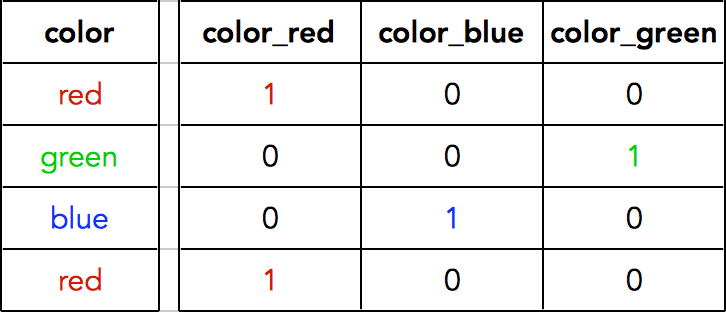
\includegraphics[width=0.5\textwidth]{capitulo_sdac/one-hot-encoding}
    \caption{Ejemplo de \emph{One-Hot Encoding}}\label{fig:onehot}
\end{figure}

\subsection{Selección de características}

Seleccionar los atributos, columnas en datos tabulares, importantes para
resolver el problema, involucra tanto conocimiento del dominio como técnico.
Elegir las mejores características asegurará que el modelo aprenda correctamente
para solucionar el problema. Difiere de la reducción de dimensionalidad en que
esta crea nuevas combinaciones de atributos para crear nuevas columnas, mientras
que la selección excluye atributos.

\subsection{Aumentación}

Para aumentar la \hyperlink{abbr}{BD} sacaremos parches de \(m \times m\),
centrados en el núcleo y rotaremos la célula un número fijo de grados. Para
encontrar el núcleo, nos auxiliaremos de la máscara para extraer el centroide de
la región del núcleo; luego exportaremos esas coordenadas a la imagen normal
para ser rotada. Para balancear la \hyperlink{abbr}{BD}, generaremos más parches
para las células normales que para las anormales. El \emph{DataFrame} es la
representación programática de una tabla de excel o archivo csv, con la mista
estructura tabular (\autoref{alg:aumentacion}). 

\begin{algorithm}[H]
    \SetAlgoLined{}
    \SetKwInOut{Input}{Input}\SetKwInOut{Output}{Output}
    \Input{Dataframe de imágenes}
    \Output{Imágenes aumentadas}
    \(m \longleftarrow 128\)
    \BlankLine{}
    \(balance \longleftarrow 0\)
    \BlankLine{}
    \For{\(row \in df\)}{    
        \BlankLine{}
        \(imagen \longleftarrow open(row[''file''])\)
        \BlankLine{}
        \uIf{\(row[''Class\_cat\_2''\)] == normal}{
            \(balance = 50\)
        }
        \uElse{
            \(balance = 18\)
        }
        \For{\(angle \in sample(balance)\)}{
            \BlankLine{}
            \(rot \longleftarrow rotate\_bound(imagen, angle)\)
            \BlankLine{}
            \(x, y \longleftarrow centro(rot)\)
            \BlankLine{}
            \(random = randint(5, 10)\)
            \BlankLine{}
            \(salida = sub\_image(rot, (x,y), angle, m, m, desp=random)\)
            \BlankLine{}
            \(salida = resize(salida, (256, 256))\)
            \BlankLine{}
        } 
    }
    \caption{Algoritmo para aumentación de datos}\label{alg:aumentacion}
\end{algorithm}

Se tomaron 50 muestras para células normales y 18 muestras para anormales de un
rango de ángulos entre 0 y 360 grados. Posteriormente se extrajo el centroide de
la imagen usando la máscara\footnote{Utilizando una técnica llamada Método de
Momentos.}. Los parches fueron extraídos de estas imágenes rotadas, la medida fue
de \(128 \times 128\) pixeles y, para asegurar cierta variación para hacer el
modelo más robusto, se desplazó el centro en el eje \(x\) y \(y\) por un número
aleatorio entre 5 y 10 pixeles. Por último se cambió el tamaño de la imagen a
\(256 \times 256\) pixeles (\autoref{fig:muestras_augment}). 
  
\begin{figure}[]
    \centering
    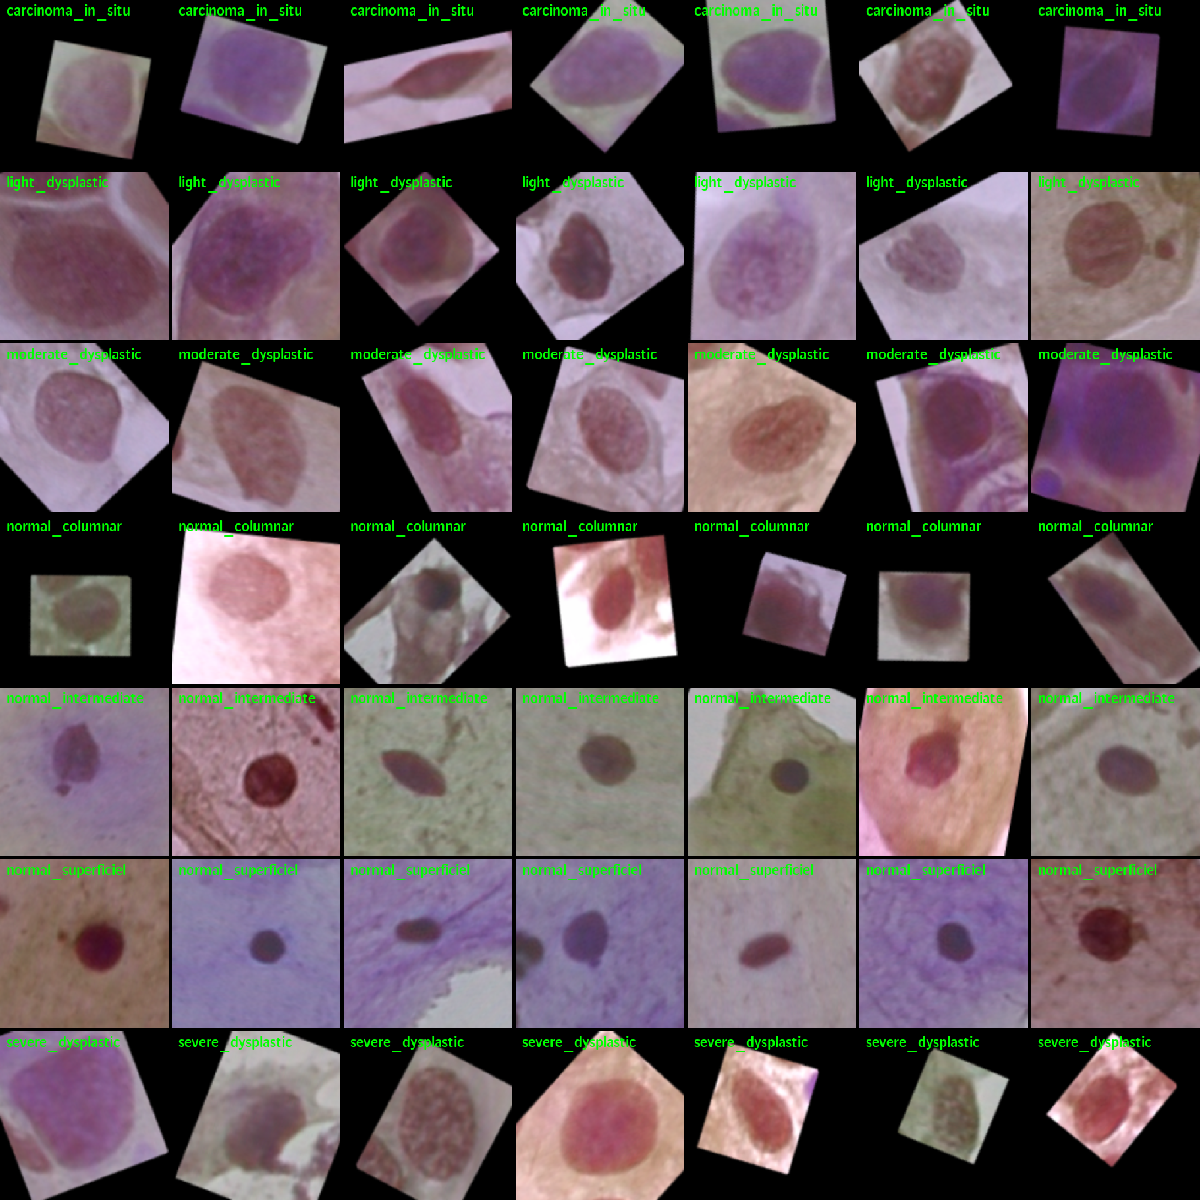
\includegraphics[width=1\textwidth]{capitulo_sdac/muestras_augment}
    \caption{Muestreo de la BD aumentada (células)}\label{fig:muestras_augment}
\end{figure}

No solo se aumentaron las imágenes de células normales, sino también las de las
máscaras (\autoref{fig:muestras_augment_masks}). Bajo el contraste de la máscara
podemos apreciar cómo las células normales presentan más regularidad en sus
estructuras y las anormales se vuelven más caóticas.

\begin{figure}[]
    \centering
    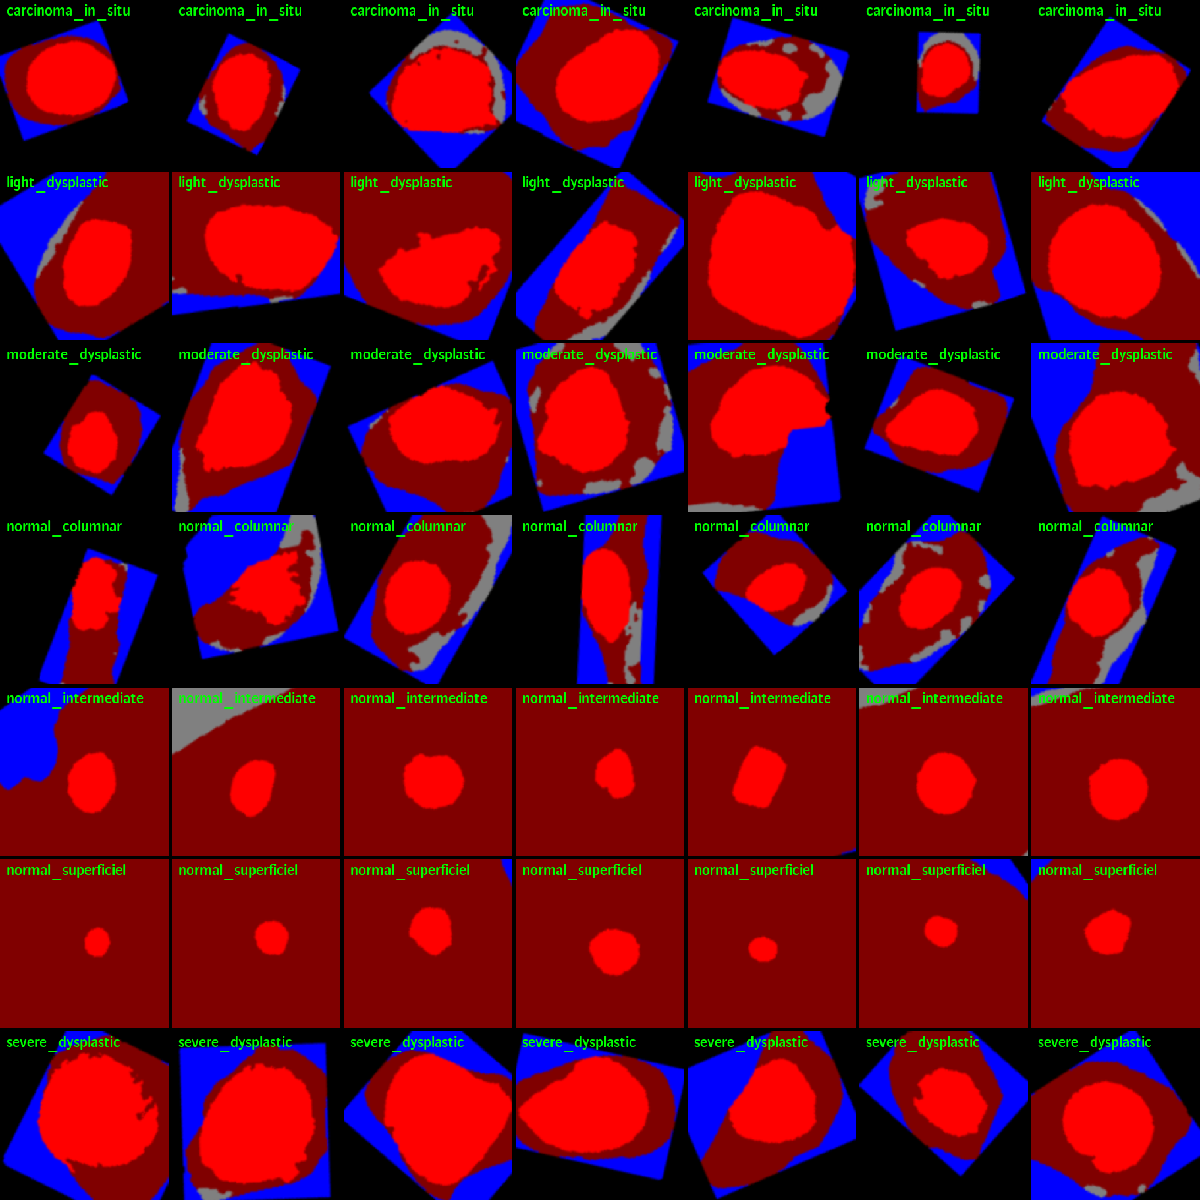
\includegraphics[width=1\textwidth]{capitulo_sdac/muestras_augment_masks}
    \caption{Muestreo de la BD aumentada (máscaras)}\label{fig:muestras_augment_masks}
\end{figure}

\subsection{Conocimiento}

Como conocimiento, tenemos una BD con imágenes variadas y aumentadas
aleatoriamente capaz de maximizar el poder de generalización de nuestro
algoritmo. Una preocupación que incluimos en el supuesto, es la de si la fase de
aumentación de datos incide en la capacidad de decisión del algoritmo. Esto es
evidente en las imágenes aumentadas, donde las partes que se añaden a la imagen
en el proceso de rotación y de cambio de tamaño se llenan con pixeles negros. 

Finalmente generamos un archivo \emph{.csv} con todas las imágenes aumentadas y su ruta
absoluta. Esto nos permitirá entrenar el modelo sin cargar todas las imágenes la
memoria, algo que sería totalmente impráctico, haciendo uso de una función que
nos permite alimentar fila por fila el archivo al algoritmo de entrenamiento.
